\clearpage


\chapter{Исследовательская часть}\label{ch:-}
В этом разделе приведен сравнительный анализ алгоритмов по времени выполнения.


\section{Технические характеристики ЭВМ}\label{sec:--2}
Все замеры проводились на ЭВМ, характеристики которой приведены ниже:
\begin{itemize}
    \item процессор: AMD Ryzen™ 7--5800H with Radeon™ Graphics × 16;
    \item ОС: 64-разрядная операционная система Ubuntu 24.04.1 LTS;
    \item оперативная память: 16,0 ГБ.
\end{itemize}


\section{Сравнение алгоритмов}
В таблице~\ref{tbl:work_time} приведено время работы алгоритмов в секундах.
Для повышения точности результатов проводилось 50 замеров.

\begin{table}[h]
    \begin{center}
        \caption{\label{tbl:work_time} Сравнение алгоритмов решения задачи коммивояжера по времени выполнения}
        \begin{tabular}{|r|r|r|}
            \hline
            Размерность матрицы & Полный перебор (сек) & Муравьиный алгоритм (сек) \\ \hline
            2                   & 0.00000              & 0.00015                   \\ \hline
            3                   & 0.00001              & 0.00027                   \\ \hline
            4                   & 0.00002              & 0.00044                   \\ \hline
            5                   & 0.00010              & 0.00062                   \\ \hline
            6                   & 0.00106              & 0.00083                   \\ \hline
            7                   & 0.00622              & 0.00113                   \\ \hline
            8                   & 0.05782              & 0.00137                   \\ \hline
        \end{tabular}
    \end{center}
\end{table}

\clearpage
На графике~\ref{grph:work_time} приведена визуализация результатов.
\begin{figure}[H]
    \centering
    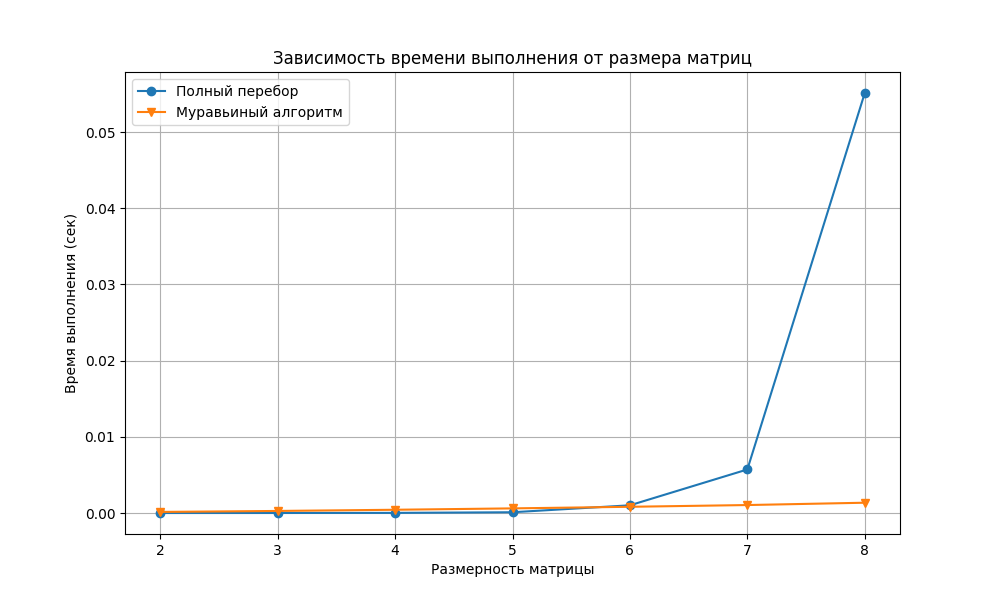
\includegraphics[width=1\linewidth]{images/execution_time_plot}
    \caption{Сравнения для каждого элемента в алгоритме полного перебора}
    \label{grph:work_time}
\end{figure}


\section{Параметризация}

Муравьиный алгоритм не гарантирует нахождение оптимального решения задачи.
Целью проведения параметризации является определение параметров, при которых муравьиный алгоритм дает наилучшие результаты.

Для параметризации в качестве критерия качества получаемого решения используется
максимальное значение, медианное и среднее арифметическое значения отклонения затрат
полученного маршрута от эталонных затрат.

Одно медианное значение, как и одно максимальное, как и одно среднее арифметическое, --- каждое получается для
серии результатов для каждого графа, для одного графа выполнено 10 запусков поиска решения муравейником.

\subsection{Класс данных}

В качестве класса данных для параметризации используются графы,
построенные на портах Атлантического, Тихого и Индийского океанов.
Всего 3 графа, представленные матрицами смежности размером 10 на 10.
Расстояния представлены в километрах. Сами расстояния были найдены при помощи приложения $Google$ $Maps{[5]}$.

\subsection*{Атлантический океан}
Порты:

\begin{enumerate}
    \item Нью Йорк (США);
    \item Норфолк (США);
    \item Чарльстон (США);
    \item Гамбург (Германия);
    \item Роттердам (Нидерланды);
    \item Ле Хавре (Франция);
    \item Ливерпуль (Великобритания);
    \item Касабланка (Марокко);
    \item Буэнос-Айрес (Аргентина);
    \item Сантос (Бразилия).
\end{enumerate}



\[
    \begin{bmatrix}
        0    & 600  & 1100 & 6600  & 6500  & 6200  & 5300  & 5800 & 8400  & 7600  \\
        600  & 0    & 630  & 6700  & 6600  & 6300  & 5400  & 6000 & 8400  & 7800  \\
        1100 & 630  & 0    & 7200  & 7100  & 6800  & 5900  & 6200 & 8000  & 7400  \\
        6600 & 6700 & 7200 & 0     & 600   & 900   & 960   & 2900 & 11700 & 10600 \\
        6500 & 6600 & 7100 & 600   & 0     & 600   & 850   & 2800 & 11600 & 10500 \\
        6200 & 6300 & 6800 & 900   & 600   & 0     & 700   & 2400 & 11500 & 10400 \\
        5300 & 5400 & 5900 & 960   & 850   & 700   & 0     & 2200 & 11400 & 10300 \\
        5800 & 6000 & 6200 & 2900  & 2800  & 2400  & 2200  & 0    & 8100  & 7600  \\
        8400 & 8400 & 8000 & 11700 & 11600 & 11500 & 11400 & 8100 & 0     & 1900  \\
        7600 & 7800 & 7400 & 10600 & 10500 & 10400 & 10300 & 7600 & 1900  & 0     \\
    \end{bmatrix}
\]

\subsection*{Тихий океан}
Порты:

\begin{enumerate}
    \item Шанхай (Китай);
    \item Пусан (Республика Корея);
    \item Йокохама (Япония);
    \item Лос Анджелес (США);
    \item Long Beach (США);
    \item Oakland (США);
    \item Ванкувер (Канада);
    \item Сиэтл (США);
    \item Манила (Филиппины);
    \item Гонконг (Китай).
\end{enumerate}


\[
    \begin{bmatrix}
        0     & 870  & 1820 & 10400 & 10450 & 9850  & 8900  & 9000  & 1840  & 1260  \\
        870   & 0    & 1100 & 9840  & 9900  & 9450  & 8200  & 8350  & 2000  & 2100  \\
        1820  & 1100 & 0    & 8800  & 8900  & 8300  & 7500  & 7600  & 3000  & 2900  \\
        10400 & 9840 & 8800 & 0     & 30    & 560   & 1700  & 1550  & 11700 & 11600 \\
        10450 & 9900 & 8900 & 30    & 0     & 640   & 1750  & 1600  & 11800 & 11700 \\
        9850  & 9450 & 8300 & 560   & 640   & 0     & 1300  & 1200  & 11500 & 11400 \\
        8900  & 8200 & 7500 & 1700  & 1750  & 1300  & 0     & 230   & 10500 & 10400 \\
        9000  & 8350 & 7600 & 1550  & 1600  & 1200  & 230   & 0     & 10400 & 10300 \\
        1840  & 2000 & 3000 & 11700 & 11800 & 11500 & 10500 & 10400 & 0     & 1500  \\
        1260  & 2100 & 2900 & 11600 & 11700 & 11400 & 10400 & 10300 & 1500  & 0     \\
    \end{bmatrix}
\]

\subsection*{Индийский океан}
Порты:

\begin{enumerate}
    \item Мумбай (Индия);
    \item Коломбо (Шри-Ланка);
    \item Карачи (Пакистан);
    \item Дербин (ЮАР);
    \item Mombasa (Кения);
    \item Perth (Австралия);
    \item Порт Лоис (Маврикий);
    \item Salalah (Оман);
    \item Дубай (ОАЭ);
    \item Сингапур (Сингапур).
\end{enumerate}

\[
    \begin{bmatrix}
        0    & 1500 & 900  & 6200 & 4600 & 7800 & 4700 & 2400 & 1920 & 3900 \\
        1500 & 0    & 2400 & 5300 & 3600 & 6700 & 3000 & 3100 & 3300 & 3300 \\
        900  & 2400 & 0    & 6400 & 4200 & 7600 & 5300 & 2450 & 1200 & 5000 \\
        6200 & 5300 & 6400 & 0    & 2400 & 6500 & 3000 & 5600 & 6600 & 7100 \\
        4600 & 3600 & 4200 & 2400 & 0    & 6500 & 1900 & 2500 & 3600 & 6300 \\
        7800 & 6700 & 7600 & 6500 & 6500 & 0    & 5800 & 8000 & 8750 & 3900 \\
        4700 & 3000 & 5300 & 3000 & 1900 & 5800 & 0    & 4600 & 5300 & 4500 \\
        2400 & 3100 & 2450 & 5600 & 2500 & 8000 & 4600 & 0    & 1000 & 5600 \\
        1920 & 3300 & 1200 & 6600 & 3600 & 8750 & 5300 & 1000 & 0    & 5800 \\
        3900 & 3300 & 5000 & 7100 & 6300 & 3900 & 4500 & 5600 & 5800 & 0    \\
    \end{bmatrix}
\]

\subsection{Результат параметризации}

В результате параметризации полечена таблица со следующими параметрами:
\begin{itemize}
    \item $\alpha$ -- коэффициент влияния феромона;
    \item $\rho$ -- коэффициент испарения феромона;
    \item дни -- число итераций;
    \item $Max$, $Med$, $Avg$ -- максимальное, медианное и среднее значение отклонения.
\end{itemize}

Далее представлен фрагмент из таблицы с наилучшими результатами~\ref{tbl:param}. Полная таблица представлена в приложении А.
\begin{longtable}{|r|r|r|r|r|r|r|r|r|r|r|r|}
    \caption{Результаты параметризации муравьиного алгоритма (начало)}\label{tbl:param}
    \\
    \hline
    \multicolumn{3}{|c|}{Параметры} & \multicolumn{3}{|c|}{Граф 1} & \multicolumn{3}{|c|}{Граф 2} & \multicolumn{3}{|c|}{Граф 3} \\
    \hline
    \multicolumn{1}{|c|}{$\alpha$} & \multicolumn{1}{|c|}{p} & \multicolumn{1}{|c|}{Дни} & \multicolumn{1}{|c|}{max} & \multicolumn{1}{|c|}{med} & \multicolumn{1}{|c|}{avg} & \multicolumn{1}{|c|}{max} & \multicolumn{1}{|c|}{med} & \multicolumn{1}{|c|}{avg} & \multicolumn{1}{|c|}{max} & \multicolumn{1}{|c|}{med} & \multicolumn{1}{|c|}{avg} \\
    \endfirsthead
    \caption{Результаты параметризации муравьиного алгоритма (продолжение)}
    \\
    \hline
    \multicolumn{3}{|c|}{Параметры}                            & \multicolumn{3}{|c|}{Граф 1}                     & \multicolumn{3}{|c|}{Граф 2}                       & \multicolumn{3}{|c|}{Граф 3}                       \\
    \hline
    \multicolumn{1}{|c|}{$\alpha$}                            & \multicolumn{1}{|c|}{p}                     & \multicolumn{1}{|c|}{Дни}                       & \multicolumn{1}{|c|}{max}                       & \multicolumn{1}{|c|}{med}                       & \multicolumn{1}{|c|}{avg}                       & \multicolumn{1}{|c|}{max}                       & \multicolumn{1}{|c|}{med}                       & \multicolumn{1}{|c|}{avg}                       & \multicolumn{1}{|c|}{max}                      & \multicolumn{1}{|c|}{med}                      & \multicolumn{1}{|c|}{avg}                      \\
    \hline
    \endhead
    \hline
    \endfoot
    \endlastfoot
    \hline
    0.5                            & 0.1                     & 200                       & 3.4                       & 1.1                       & 1.3                       & 4.0                       & 1.4                       & 1.6                       & 39.0                      & 23.0                      & 22.0                      \\
    \hline \
    0.5                            & 0.1                     & 300                       & 6.0                       & 1.2                       & 2.3                       & 2.0                       & 0.0                       & 0.4                       & 32.0                      & 21.0                      & 16.7                       \\
    \hline \
    0.5                            & 0.1                    & 400                       & 2.4                       & 0.4                       & 0.8                       & 2.0                       & 0.0                       & 0.3                       & 30.0                      & 16.6                      & 15.5                      \\
    \hline \
    0.5                            & 0.1                    & 500                       & 3.0                       & 1.9                       & 1.4                       & 0.8                       & 0.0                       & 0.2                       & 21.0                      & 10.0                      & 9.6                      \\
    \hline \
    0.5 & 0.25 & 100 & 6.4 & 3.4 & 3.2 & 7.8 & 2.0 & 2.4 & 44.0 & 29.6 & 26.0 \\
    \hline
%    0.5 & 0.25 & 200 & 5.7 & 2.0 & 2.6 & 2.0 & 0.0 & 0.4 & 44.0 & 29.0 & 26.2 \\
    \
\end{longtable}

\section*{Вывод}

В результате исследования по времени было установлено, что при размерности матрицы <= 6,
муравьиный алгоритм и алгоритм полного перебора выполняют задачу примерно за одинаковое время.
При большей размерности (7 и более) муравьиный алгоритм работает примерно в 6 раз быстрее.

Результаты параметризации показали, что наилучшей комбинацией параметров для муравьиного алгоритма будет
$\alpha$ = 0.5, $\rho$ = 0.1, $t\_{max}$ = 500.

\clearpage